\chapter{From LMS to Deep Learning}
\section{LMS of zero-mean time-series}
The time-series signal is non-stationary data, which can be analysed by the LMS algorithm. The algorithm is used to predict one-step value based on the previous four values $y[n-4]$, $y[n-3]$, $y[n-2]$ and $y[n-1]$. As shown in Fig.\ref{fig:4_1_a}(a), the time-series is non-linear and zero mean. The performance of the basic LMS algorithm is illustrated in Fig.\ref{fig:4_1_a}(b). The predicted time-series is zero-mean as well. However, the predicted series do not capture perfectly of the original at the beginning part. After 400 time index, the predicted series converge with small difference with true series. In order to evaluate the performance appropriately, the metrics of mean squared error (MSE) and prediction gain ($R_p$) are measured. The MSE should be close to zero while the gain should be as large as possible. As to the LMS algorithm, the MSE is 16.032$dB$ with $R_p=5.196$, which performs inexpressively to some extent.
\begin{figure}[htb]
     \centering
     \hspace{0.4cm}
     \begin{subfigure}[b]{0.4\textwidth}
         \centering
         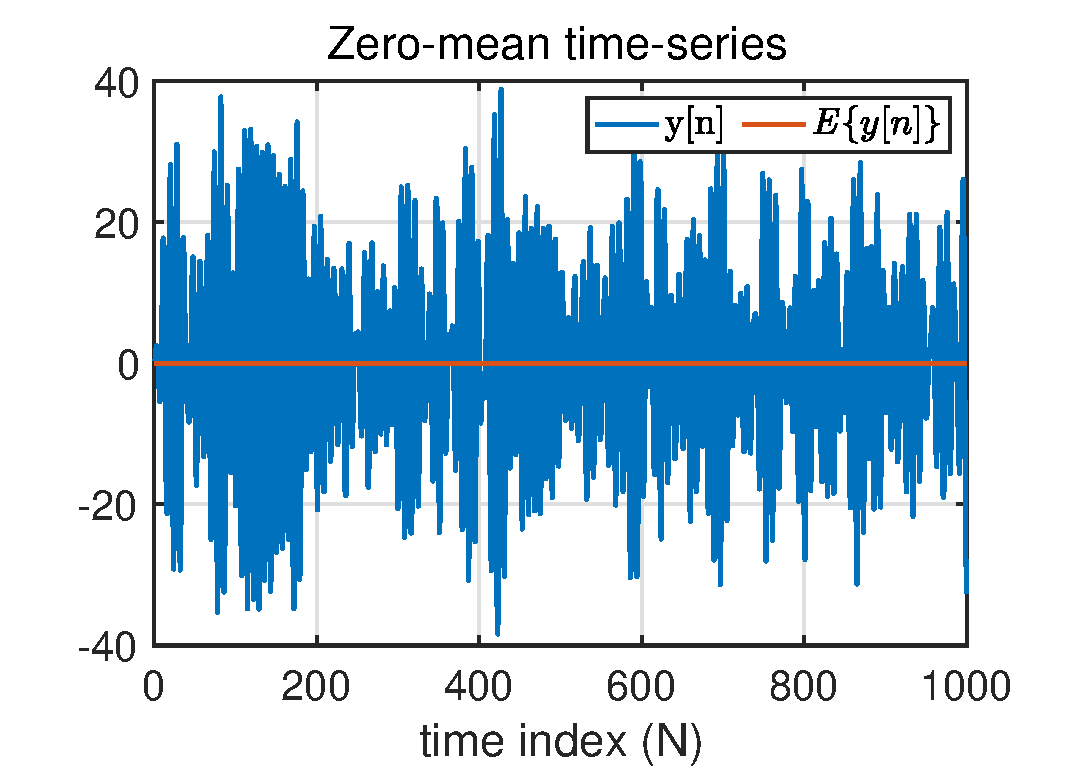
\includegraphics[width=\textwidth]{fig/4/41a1.eps}
     \end{subfigure}
    \hspace{0.4cm}
     \begin{subfigure}[b]{0.4\textwidth}
         \centering
         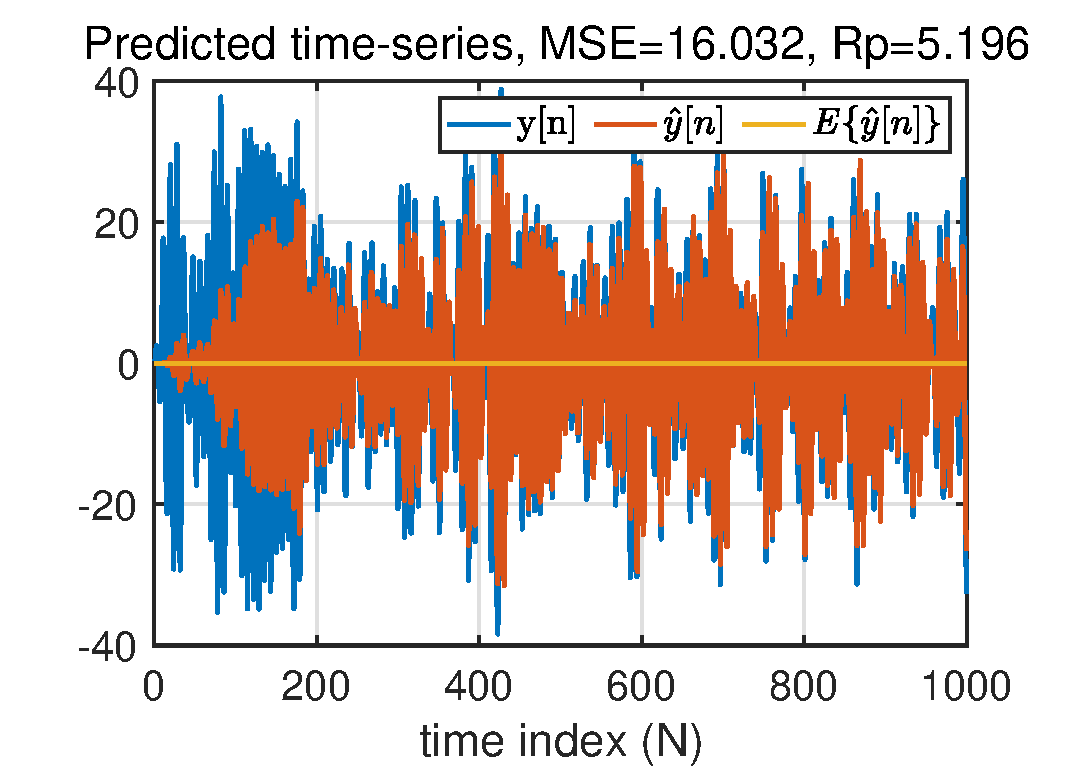
\includegraphics[width=\textwidth]{fig/4/41a2.eps}
     \end{subfigure}
     \caption{LMS: zero mean time-series one-step prediction}
     \label{fig:4_1_a}
\end{figure}
\section{Activation function of predicted series}
\begin{figure}[htb]
     \centering
     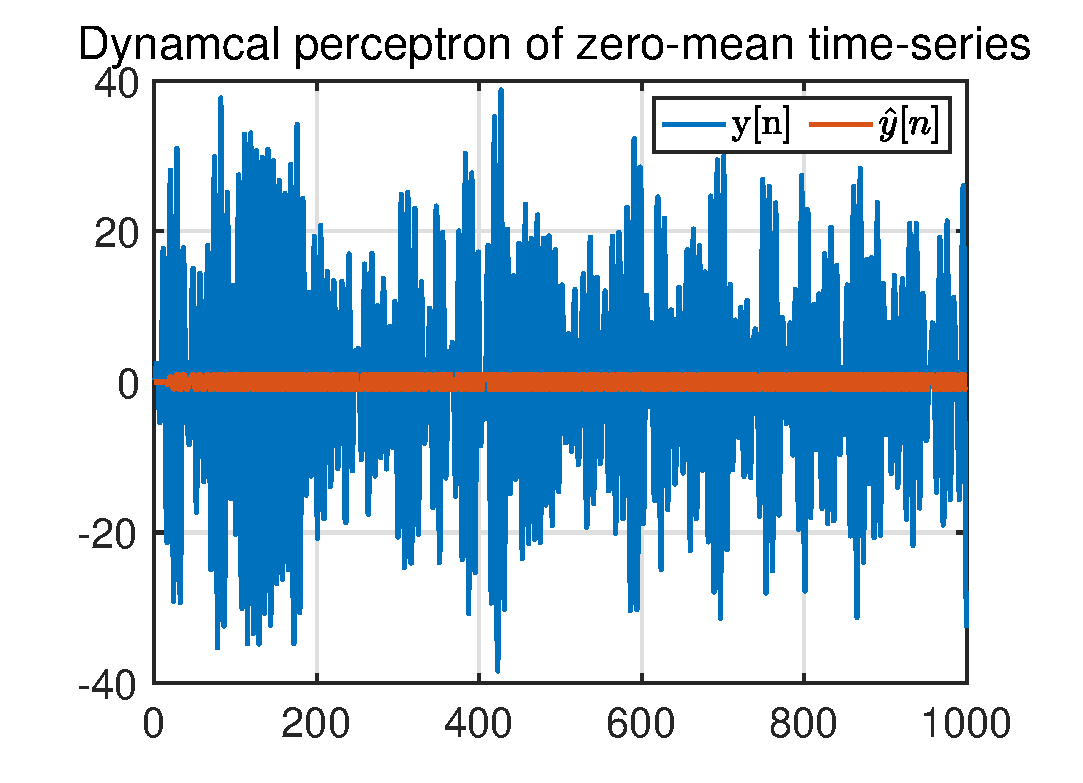
\includegraphics[width=0.4\textwidth]{fig/4/42.eps}
     \caption{Dynamical perceptron: zero mean time-series one-step prediction}
     \label{fig:4_2}
\end{figure}
\noindent
Due to the non-linearity of most of real-life data, the activation function \texttt{tanh} is applied to the each step of AR(4) process, which can be expressed as 
\begin{align}
\hat y[n]&=tanh(\mathbf{w^Ty})\label{eq:act}\\
\text{where}\quad \mathbf{y}&=[y[n-4], y[n-3], y[n-2], y[n-1]]\notag
\end{align}
Fig.\ref{fig:4_2} depicts the output using activation function against the original time-series. It is obvious that using \texttt{tanh} is inappropriate to predict the time-series data. The reason is that the range of \texttt{tanh} lies in $(-1,1)$ whereas the zero-mean time-series is bounded in $(-40,40)$. Therefore, in order to appropriately predict the series, the activation function need to be scaled.
\section{Scaled activation function}
As analysis previous, scaling the activation function expresses in Eq.\ref{eq:act} by factor $a$. Fig.\ref{fig:4_3_a} illustrates the performance of varying $a$ with zero-mean data. For a small value of $a=20$, the predicted $\hat y[n]$ is still lower than the range of the desired data. Thus, the MSE is extreme large than the standard LMS algorithm. However, the maximum range of prediction is restricted by activation function, leading to small variance of error. Thus, the prediction gain $R_p$ is larger than the LMS. With incremental of $a$ up to 80, the MSE is getting to decrease, corresponding to increasing predict gain. However, if the value of $a$ is over 80, the prediction is overshooting to the true data, resulting in decreasing $R_p$ and increasing MSE. In conclusion, the optimal range of $a$ for predictinng zero mean data is $70\sim80$.
\begin{figure}[htb]
     \centering
     \hspace{-0.4cm}
     \begin{subfigure}[b]{0.33\textwidth}
         \centering
         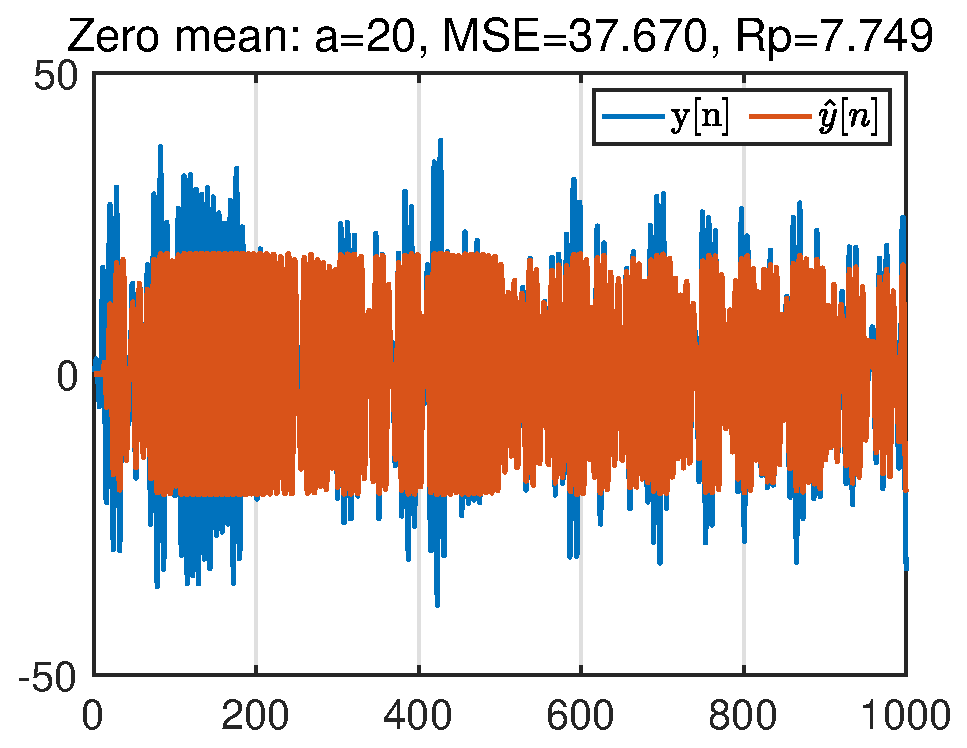
\includegraphics[width=\textwidth]{fig/4/43a1.eps}
     \end{subfigure}
    \hspace{-0.2cm}
     \begin{subfigure}[b]{0.33\textwidth}
         \centering
         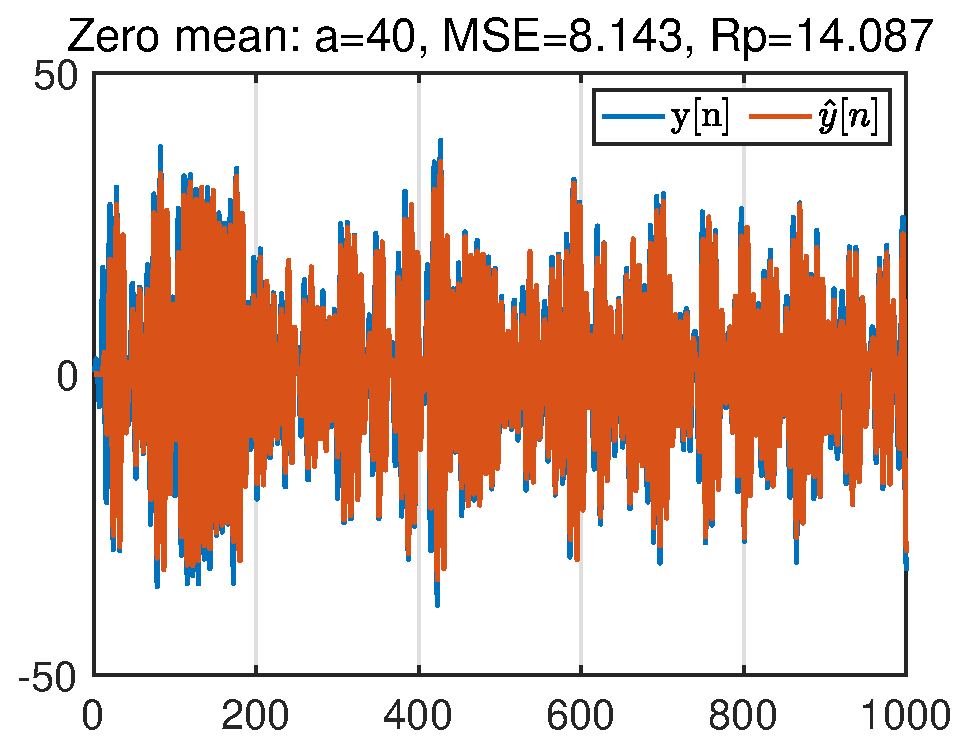
\includegraphics[width=\textwidth]{fig/4/43a2.eps}
     \end{subfigure}
    \hspace{-0.2cm}
     \begin{subfigure}[b]{0.33\textwidth}
         \centering
         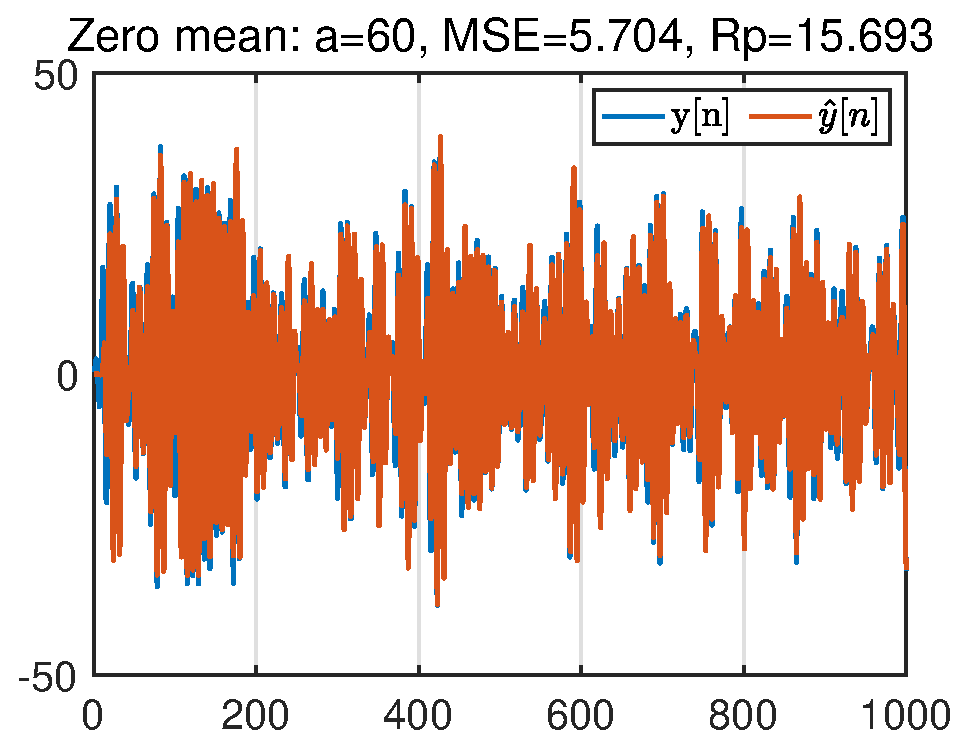
\includegraphics[width=\textwidth]{fig/4/43a3.eps}
     \end{subfigure}
     \\
     \hspace{-0.4cm}
     \begin{subfigure}[b]{0.33\textwidth}
         \centering
         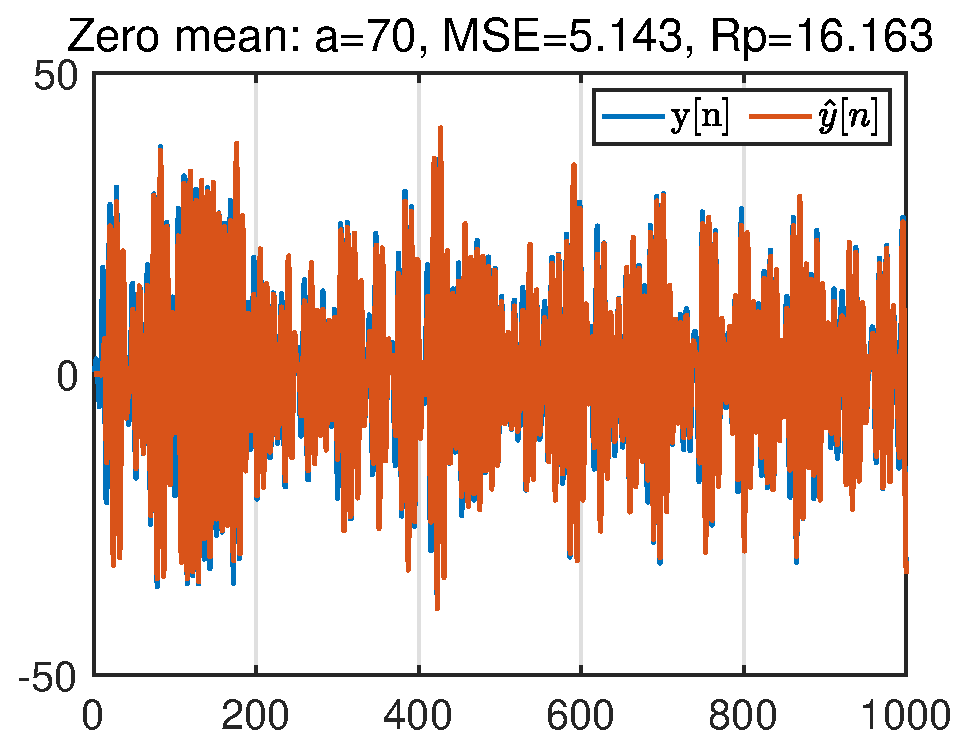
\includegraphics[width=\textwidth]{fig/4/43a4.eps}
     \end{subfigure}
    \hspace{-0.2cm}
     \begin{subfigure}[b]{0.33\textwidth}
         \centering
         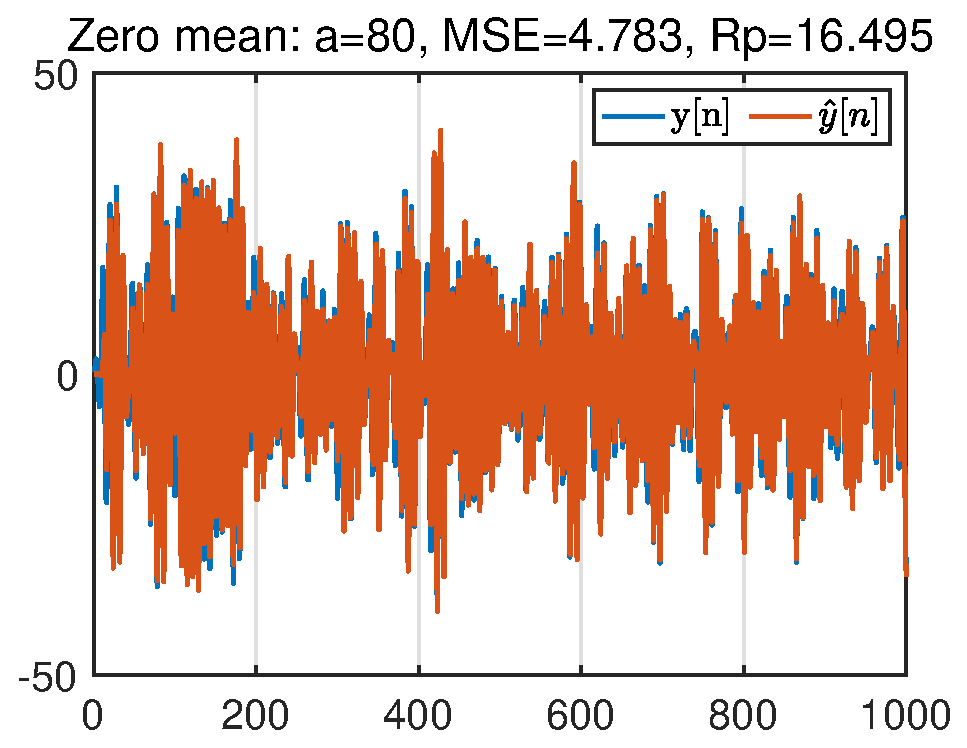
\includegraphics[width=\textwidth]{fig/4/43a5.eps}
     \end{subfigure}
    \hspace{-0.2cm}
     \begin{subfigure}[b]{0.33\textwidth}
         \centering
         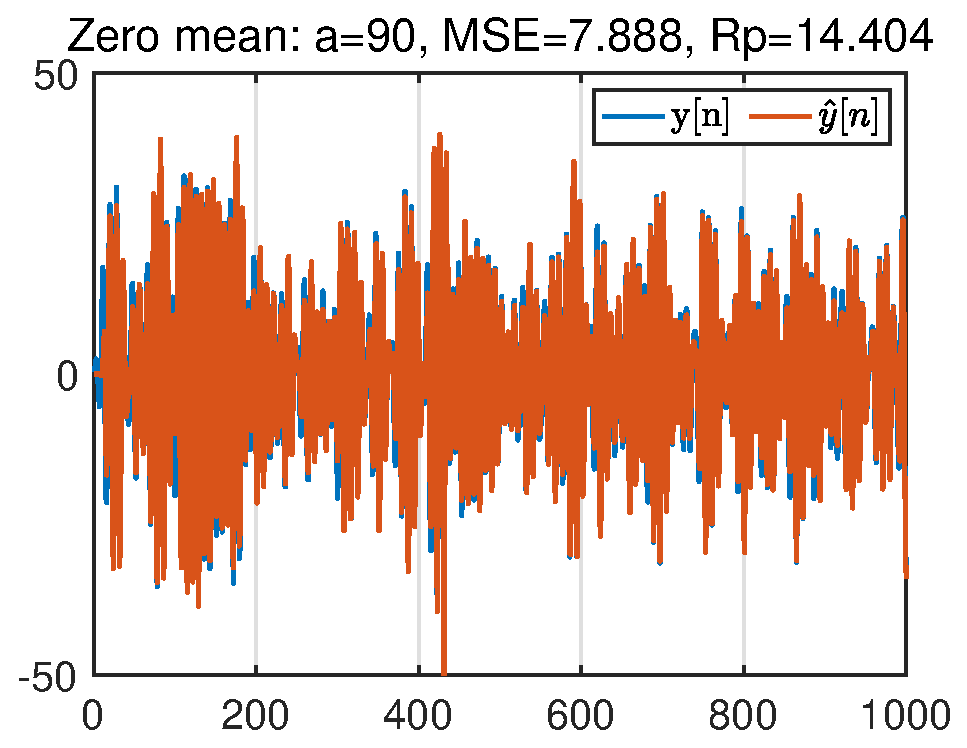
\includegraphics[width=\textwidth]{fig/4/43a6.eps}
     \end{subfigure}
       \caption{Scaled \texttt{tanh}: Prediction of zero mean data}
        \label{fig:4_3_a}
\end{figure}\\
In addition, it is harder to predict the none-zero mean data as shown in Fig.\ref{fig:4_3_b}, which presents in the larger MSE and smaller $R_p$. However, the optimal range of $a$ for non-zero mean prediction is $40\sim 50$.
\begin{figure}[htb]
     \centering
     \hspace{-0.4cm}
     \begin{subfigure}[b]{0.33\textwidth}
         \centering
         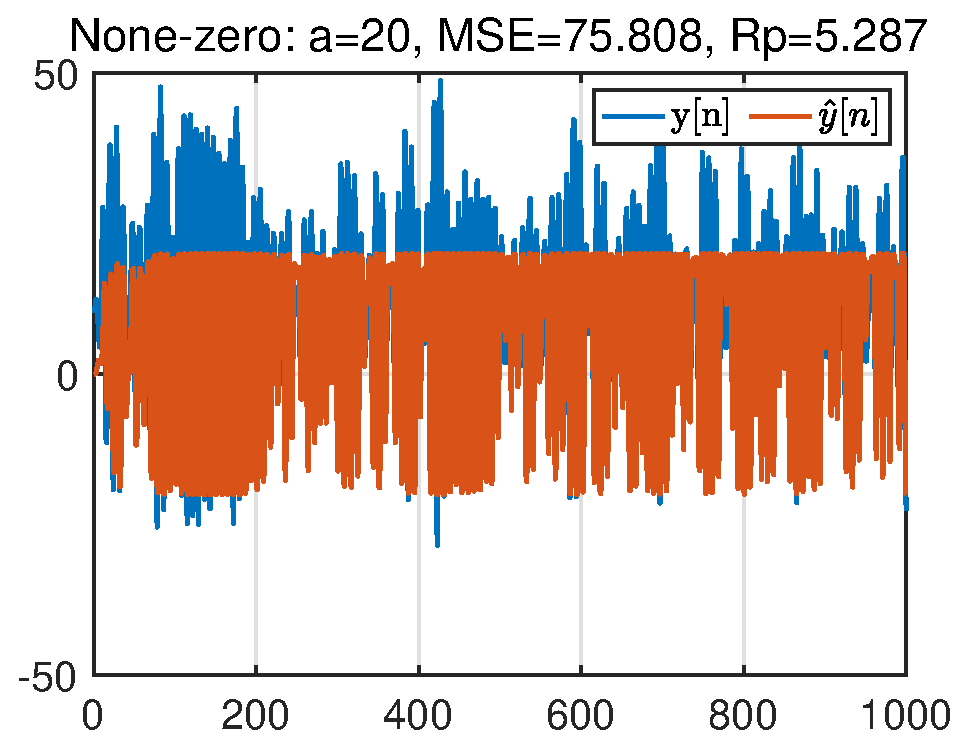
\includegraphics[width=\textwidth]{fig/4/43b1.eps}
     \end{subfigure}
    \hspace{-0.2cm}
     \begin{subfigure}[b]{0.33\textwidth}
         \centering
         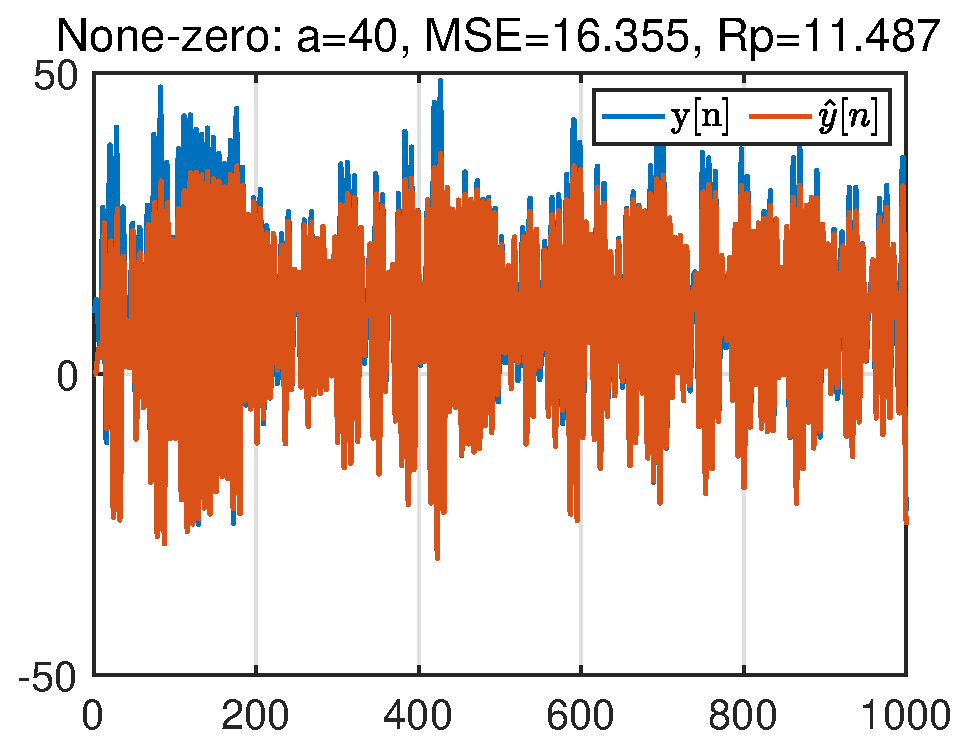
\includegraphics[width=\textwidth]{fig/4/43b2.eps}
     \end{subfigure}
    \hspace{-0.2cm}
     \begin{subfigure}[b]{0.33\textwidth}
         \centering
         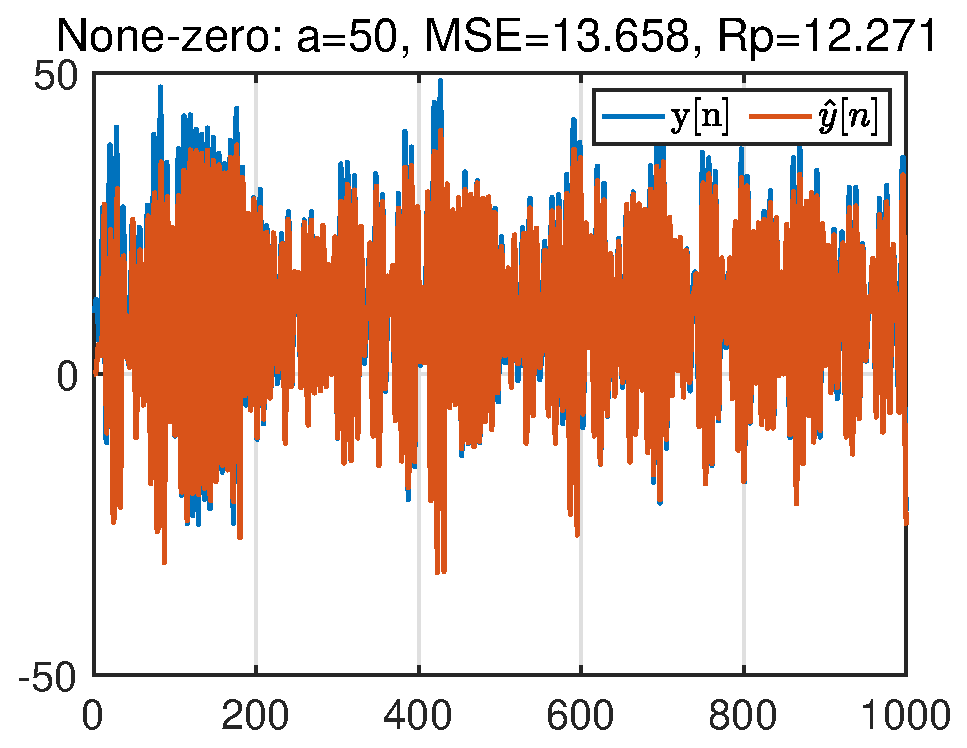
\includegraphics[width=\textwidth]{fig/4/43b3.eps}
     \end{subfigure}
     \\
     \hspace{-0.4cm}
     \begin{subfigure}[b]{0.33\textwidth}
         \centering
         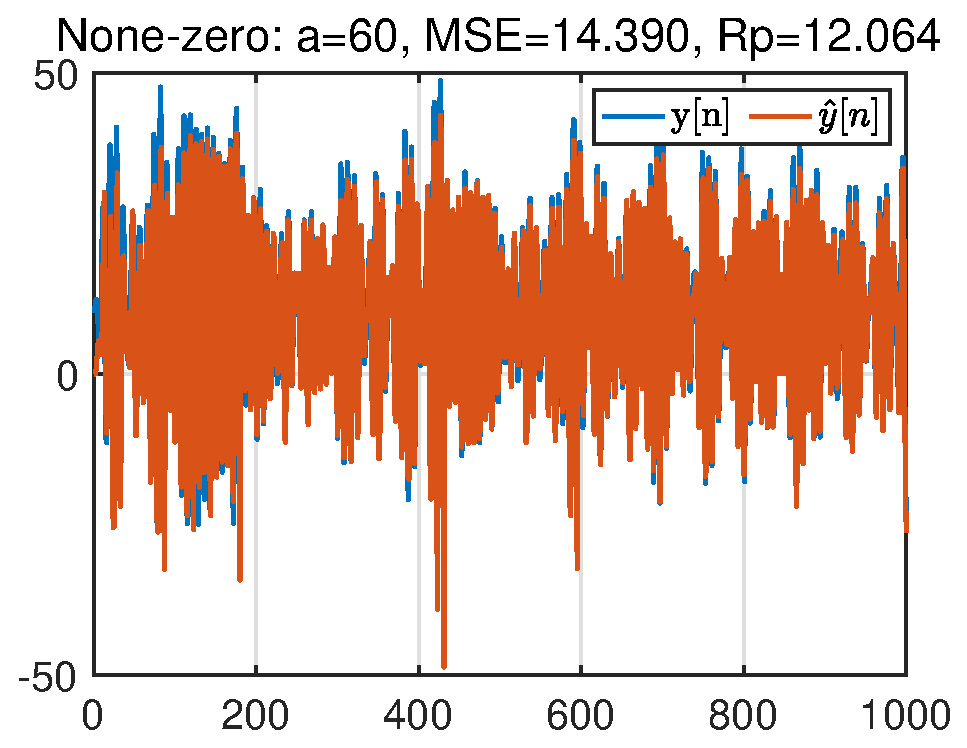
\includegraphics[width=\textwidth]{fig/4/43b4.eps}
     \end{subfigure}
    \hspace{-0.2cm}
     \begin{subfigure}[b]{0.33\textwidth}
         \centering
         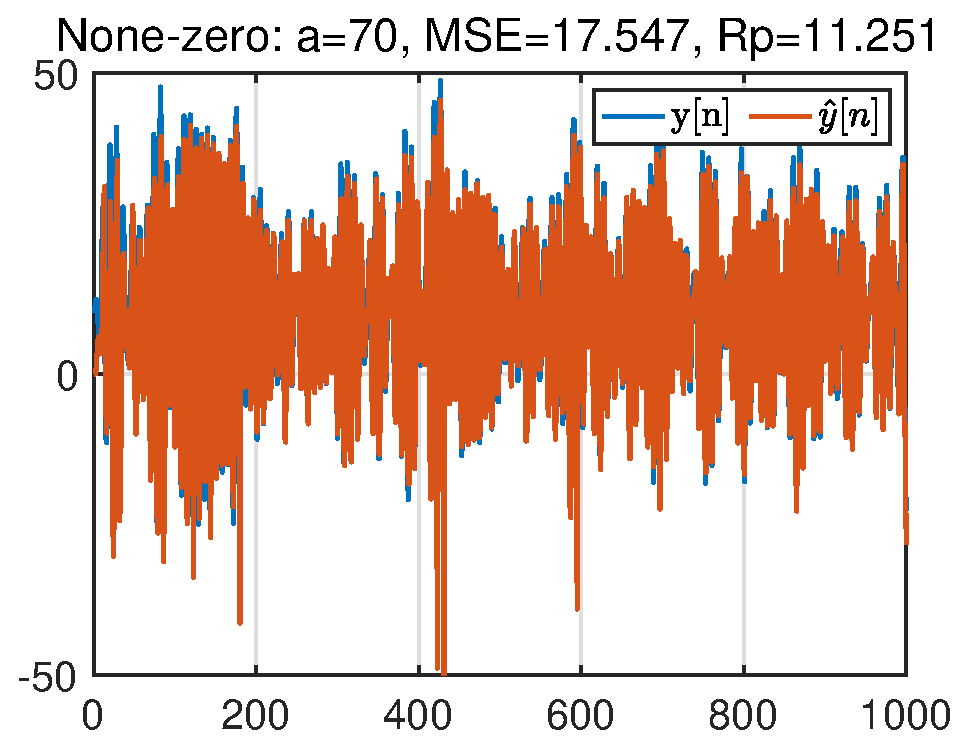
\includegraphics[width=\textwidth]{fig/4/43b5.eps}
     \end{subfigure}
    \hspace{-0.2cm}
     \begin{subfigure}[b]{0.33\textwidth}
         \centering
         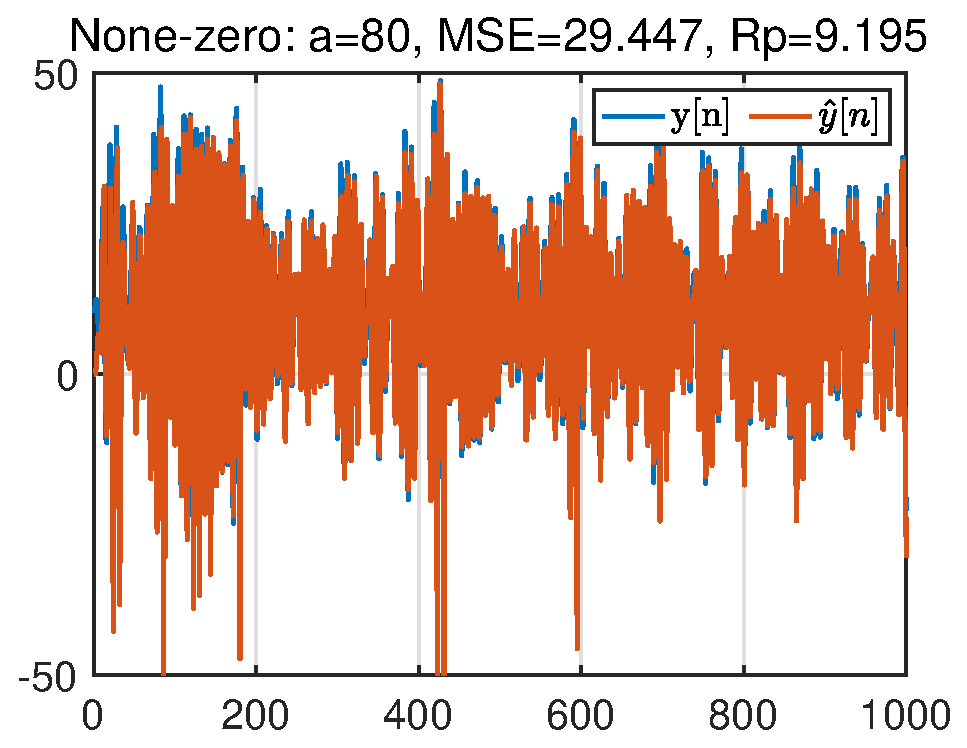
\includegraphics[width=\textwidth]{fig/4/43b6.eps}
     \end{subfigure}
       \caption{Scaled \texttt{tanh}: Prediction of none-zero mean data}
        \label{fig:4_3_b}
\end{figure}
\section{None-linearity prediction with bias}
Previous work is based on the zero mean time-series to make one-step ahead prediction. By adding a bias $b$ for the activation function, expressed as $tanh(\mathbf{w}^T\mathbf{x}+b)$, the model can account for the mean automatically. Due to the small learning rate, the performances with bias are similar to the one without bias if only one epoch experiment is implemented. Thus, 100 number of epochs are used in order to continuously update weight. Fig.\ref{fig.bia} plots the MSE curves with or without bias for 100 epochs learning. Same performances are obtained at the beginning of training. Both of curves are rapidly plummet at first epochs and then slightly decrease up to convergence. Overall, the model with bias outperform the one without bias which converges after 60 epochs. Fig.\ref{fig.biasplot} shows the prediction of last epoch with bias against with the original non-zero mean series. Compared with the plots in Fig.\ref{fig:4_3_b} with amplitude $a=50$, the MSE reduces approximately in a half and prediction gain increases as well.
\begin{figure}[htb]
     \centering
     \hspace{0.4cm}
     \begin{subfigure}[b]{0.4\textwidth}
         \centering
         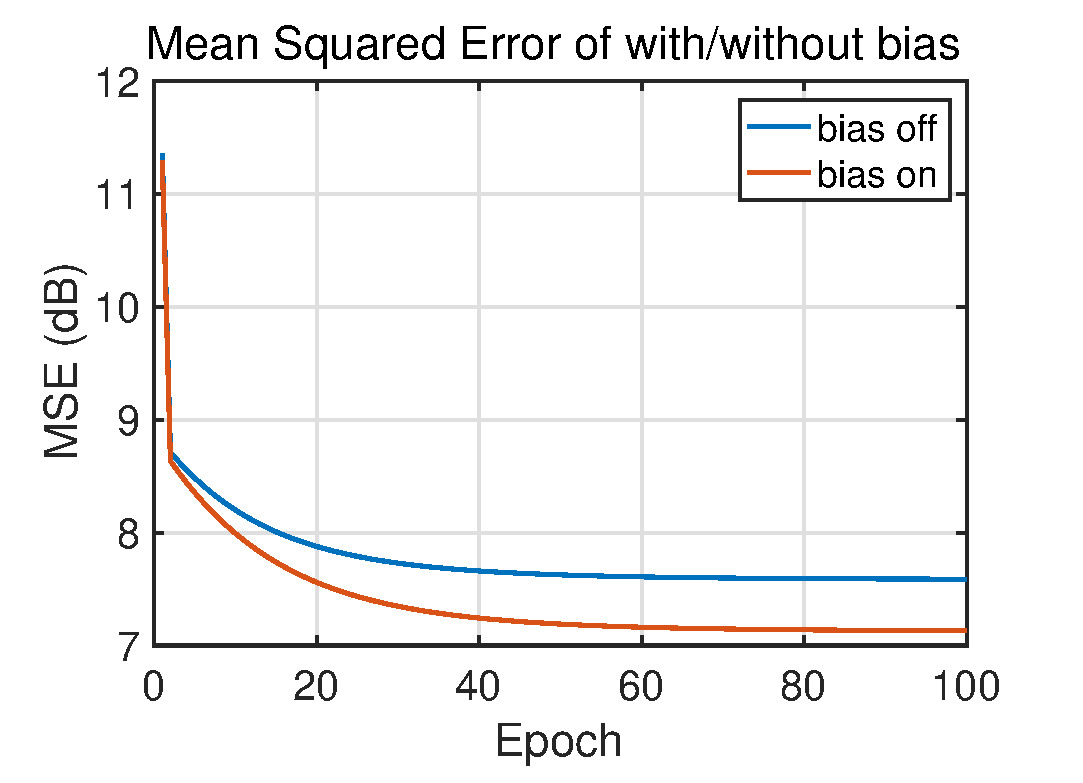
\includegraphics[width=\textwidth]{fig/4/44a2.eps}
         \caption{Prediction MSE of 100 epochs}
         \label{fig.bia}
     \end{subfigure}
    \hspace{0.4cm}
     \begin{subfigure}[b]{0.4\textwidth}
         \centering
         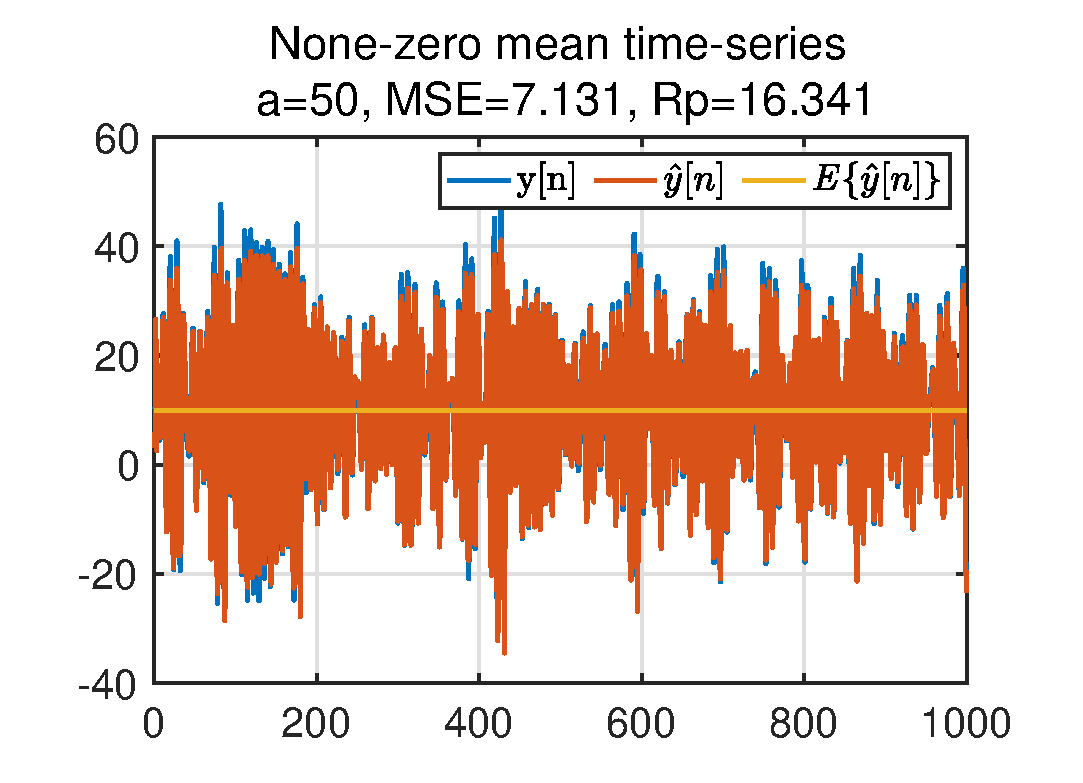
\includegraphics[width=\textwidth]{fig/4/44a1.eps}
          \caption{The last epoch prediction}
         \label{fig.biasplot}
     \end{subfigure}
     \caption{\texttt{tanh} with bias: None-zero mean time-series one-step prediction}
     \label{fig:4_4}
\end{figure}
\section{Prediction with initialized weight}
As to the LMS algorithm, the model cannot capture the original time-series at the beginning, which causes a long time to converge. Fig.\ref{fig:4_5}(a) illustrates the standard LMS prediction for non-zero mean which performs dissatisfactory with quite large error and insignificant prediction gain. The reason is that the initial weights are assumed to zero, which introduces difficulties to predict the non-zero mean data. Fig.\ref{fig:4_5} depicts the performance of training initial weights. After training the first 20 data samples for 100 epochs, the initial weights are obtained which can speed up the learning process. With the pre-trained initial weights, the model perform better than training model after 100 epoch, with smaller MSE = 5.162 and slightly larger $R_p=16.342$. 
\begin{figure}[htb]
     \centering
     \hspace{0.4cm}
     \begin{subfigure}[b]{0.4\textwidth}
         \centering
         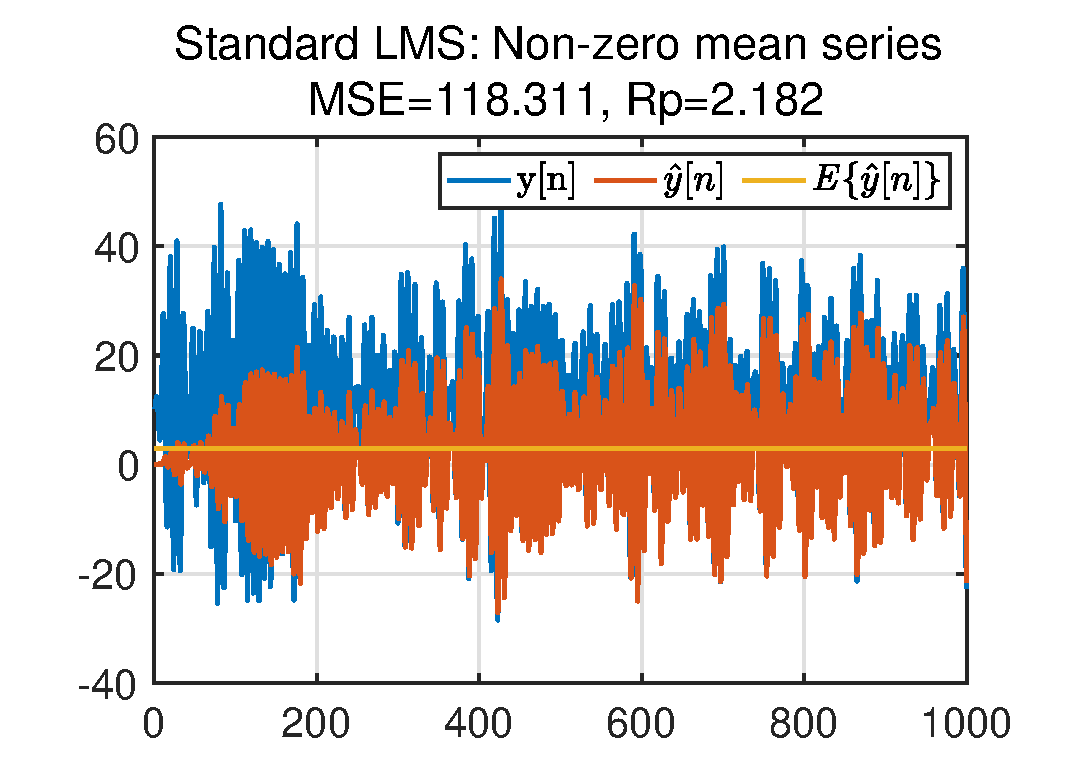
\includegraphics[width=\textwidth]{fig/4/45a1.eps}
     \end{subfigure}
    \hspace{0.4cm}
     \begin{subfigure}[b]{0.4\textwidth}
         \centering
         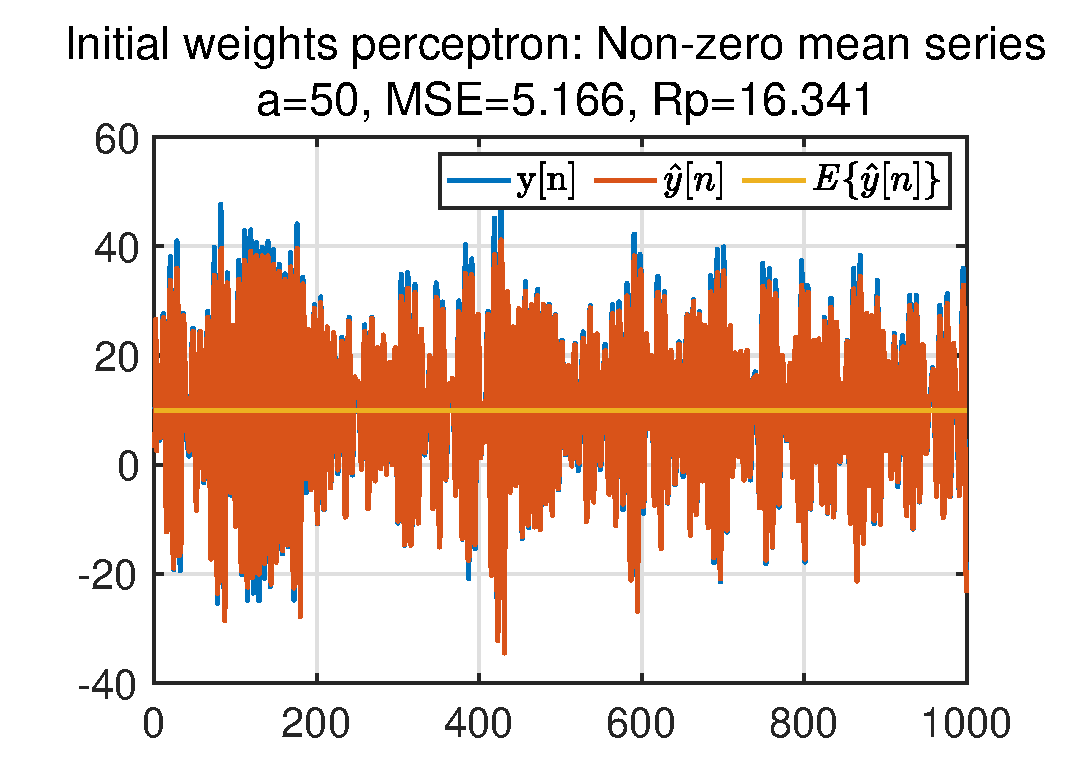
\includegraphics[width=\textwidth]{fig/4/45a2.eps}
     \end{subfigure}
     \caption{Standard LMS and Dynamical perceptron: zero mean time-series prediction}
     \label{fig:4_5}
\end{figure}
\section{Back-propagation of Deep Network}
For deep network, the neurons at each layers are fully connected with all inputs at last layer and outputs at next layer. And the weights can be expressed as:
\begin{align}
\mathbf{w}^{l}\Rightarrow w_{ij}^{(l)}\left\{
             \begin{array}{lr}
             1\leqslant l \leqslant L\text{ layers;}\\
             1\leqslant i \leqslant d^{(l-1)}\text{ inputs;} \\
             1\leqslant j \leqslant d^{(l)}\text{ outputs;} \\
             \end{array}
\right.\\
d\text{ is neuron number at each layer}\notag
\end{align}
Thus, the weighted output on each neuron position is calculated by summing all weighted inputs with activation function.
\begin{align}
z_{j}^l &=\sigma(w^l_{ij}a^{l-1}_{ij}+w^l_{i0})\\
\mathbf z^l &=\sigma(\mathbf w^l \mathbf a^{l-1}+w^l_{i0})
\end{align}
Therefore, set the weights randomly and the forward propagation process of the first iteration is finished. However, back-propagation of weights and bias need loss function, generally mean squared error, to calculated the gradient as shown below.
\begin{align}
E=\mathbb {E}\{\|x[n]-\hat x[n]\|^2 \}
\end{align}
Therefore, the error for the output $\delta^l_j$ can be expressed as
\begin{align}
\delta^l_j&=\frac{\partial E}{\partial z^l_j}\notag\\
&=\sum_i\frac{\partial z_i^{l+1}}{\partial z^l_j}\delta_i^{l+1}\notag\\
&=\sum_i w_{ij}^{l+1}\delta^{l+1}_i\sigma'(z^l_j)
\end{align}
In addition, the output error is corresponding to the previous weights. Thus, the gradient of weight is
\begin{align}
\frac{\partial E}{\partial w^l_{ij}}=a_{i}^{l-1}\delta_j^l
\end{align}
Therefore, the weight can be updated by
\begin{align}
w_{ij}=w_{ij}-\eta\frac{\partial E}{\partial w^l_{ij}}=w_{ij}-\eta a_{i}^{l-1}\delta_j^l
\end{align}
\section{Deep Network}
There are 10 sinusoidal waves with different frequency and amplitude as the linear inputs. The output $y[n]$ after applying activation function to $\mathbf x[n]$ is highly non-linear as shown in Fig.\ref{fig:4_7_1}. With the default parameters, three model, specifically in single neuron with linear and \texttt{tanh} function, deep network with \texttt{relu}, are used to train and test to evaluate their performance. 
\begin{figure}[htb]
     \centering
     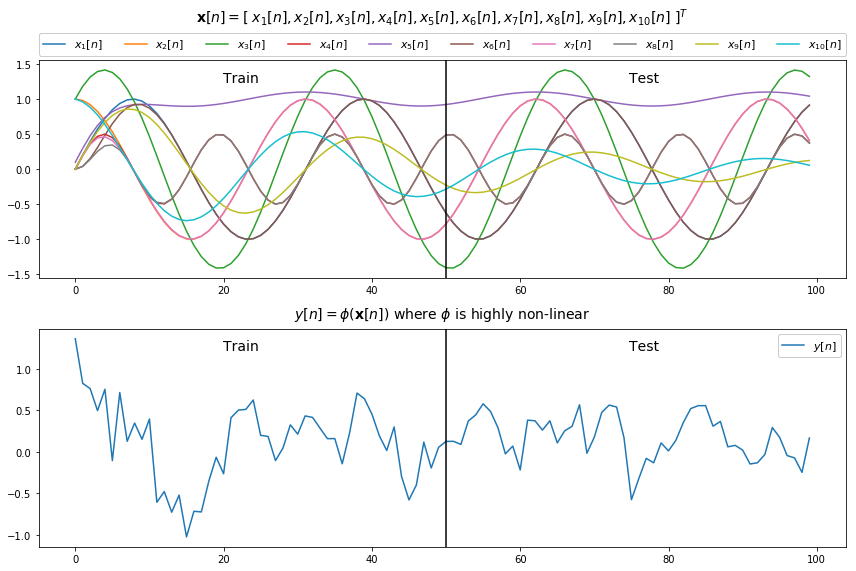
\includegraphics[width=0.7\textwidth]{fig/4/47a1.png}
     \caption{Harmonics sine waves and non-linear data with noise}
     \label{fig:4_7_1}
\end{figure}\\
Fig.\ref{fig:4_7_2} shows the regression curves of these three models. The models use single neutron have similar performance, whose predictions are still linear. As to the deep network, this model can predict non-linear curve and the trend of the data is generally predicted. However, the performance is still insignificant which may be caused by the power of noise.
\begin{figure}[htb]
     \centering
     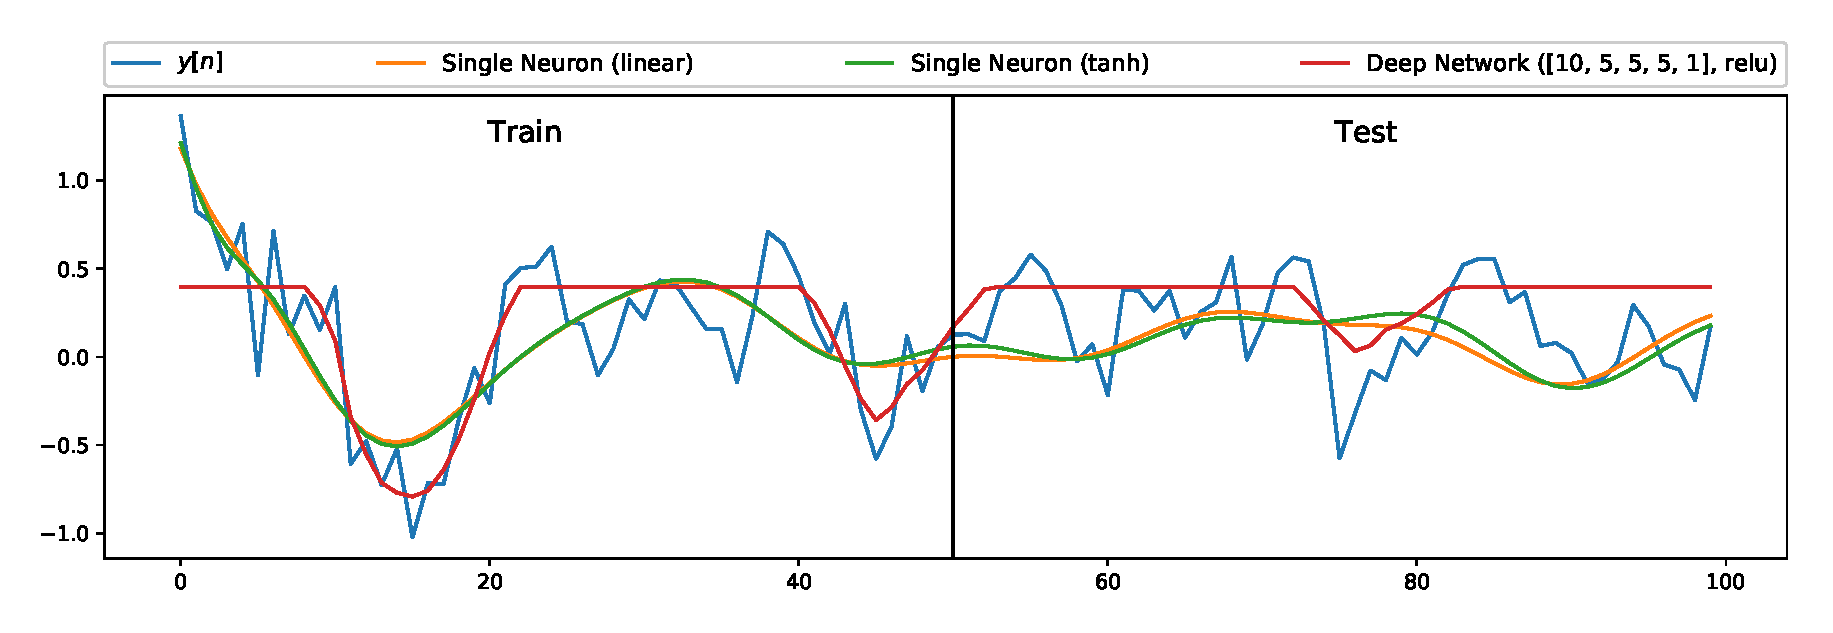
\includegraphics[width=0.7\textwidth]{fig/4/47a2.eps}
     \caption{Performance of three models}
     \label{fig:4_7_2}
\end{figure}\\
Fig.\ref{fig:4_7_3} shows the train error and test error for each model. The single neuron model learning curve rapidly decrease and then keep flat. While the test error of deep network starts at lower point and then converges to a slightly lower value. However, the single neuron models converge much more rapidly than the deep network, since their architectures are simple which are easily to be trained.
\begin{figure}[htb]
     \centering
     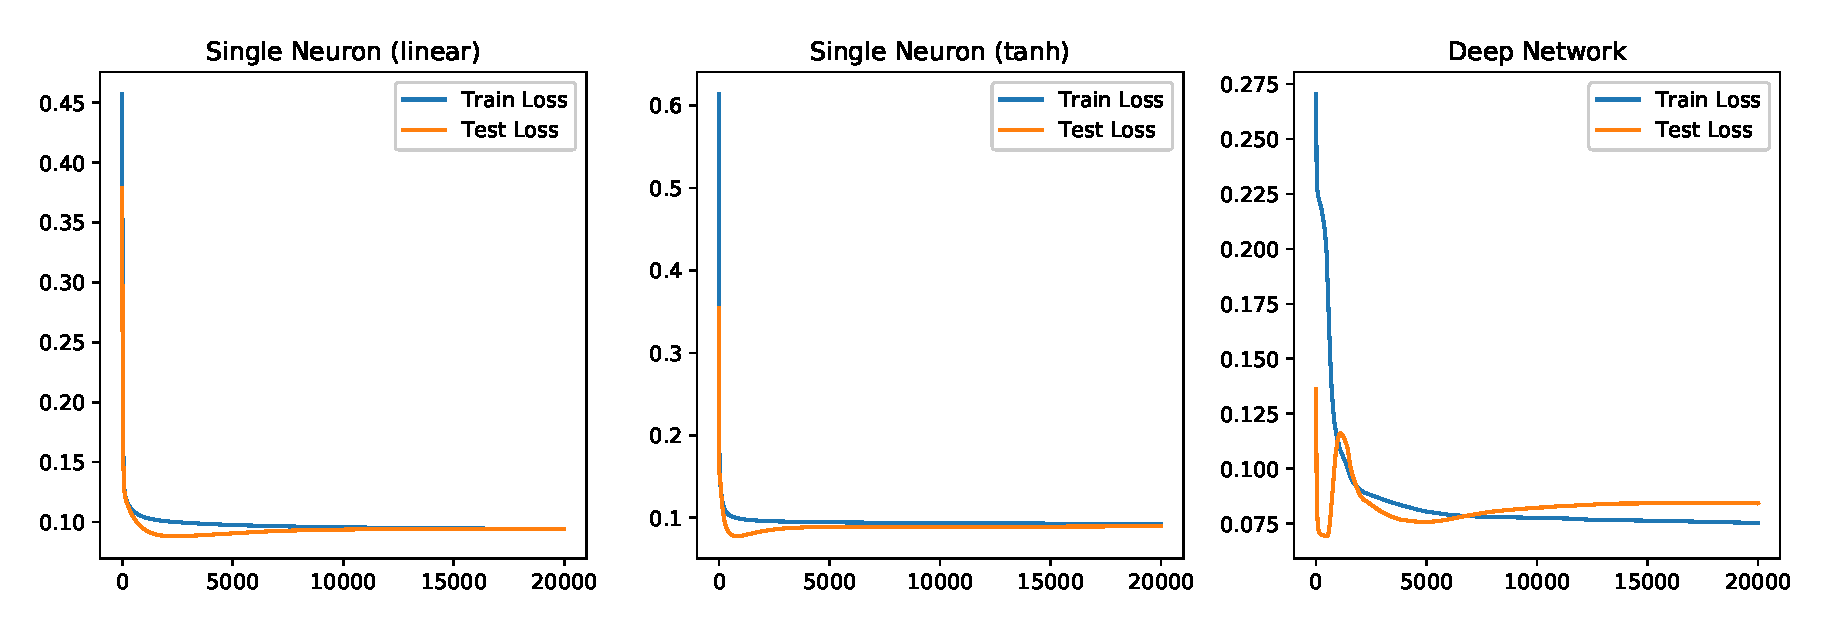
\includegraphics[width=0.8\textwidth]{fig/4/47a3.eps}
     \caption{Learning curves of three models}
     \label{fig:4_7_3}
\end{figure}
\newpage
\section{Noise power and drawbacks of Deep Network}
Experiments are repeated by changing different power of noise which are $\sigma^2=$ 0, 0.01, 0.2. Fig.\ref{fig:4_8_b} shows the predictions and learning curves with $\sigma^2=0$. The model of deep network outperform during training and testing. The series is accurately captured in training and acceptable error in testing. However, the single neutron models can not predict non-linear series as well. 
\begin{figure}[htb]
     \centering
     \begin{subfigure}[b]{0.8\textwidth}
         \centering
         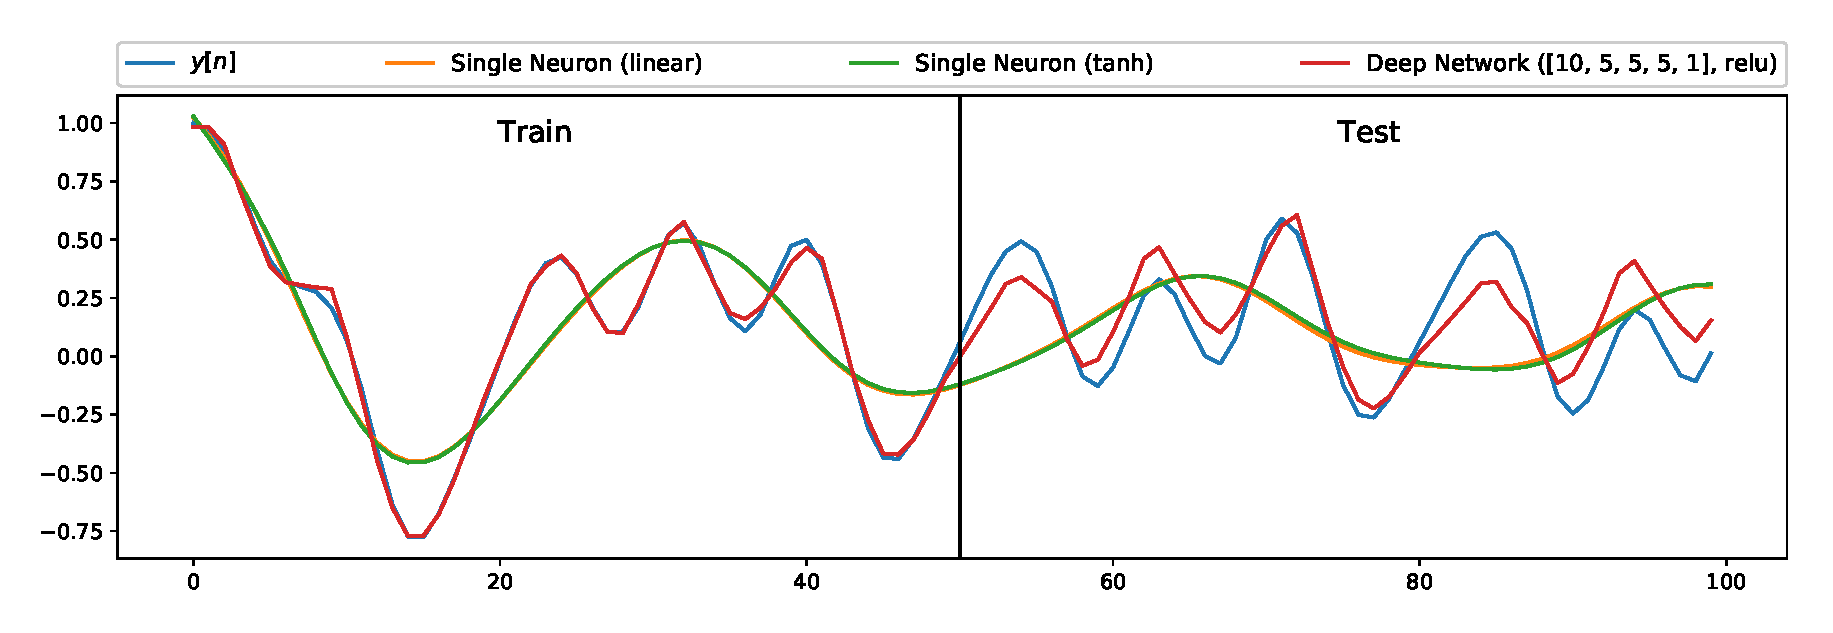
\includegraphics[width=\textwidth]{fig/4/48b1.eps}
     \end{subfigure}
     \begin{subfigure}[b]{0.8\textwidth}
         \centering
         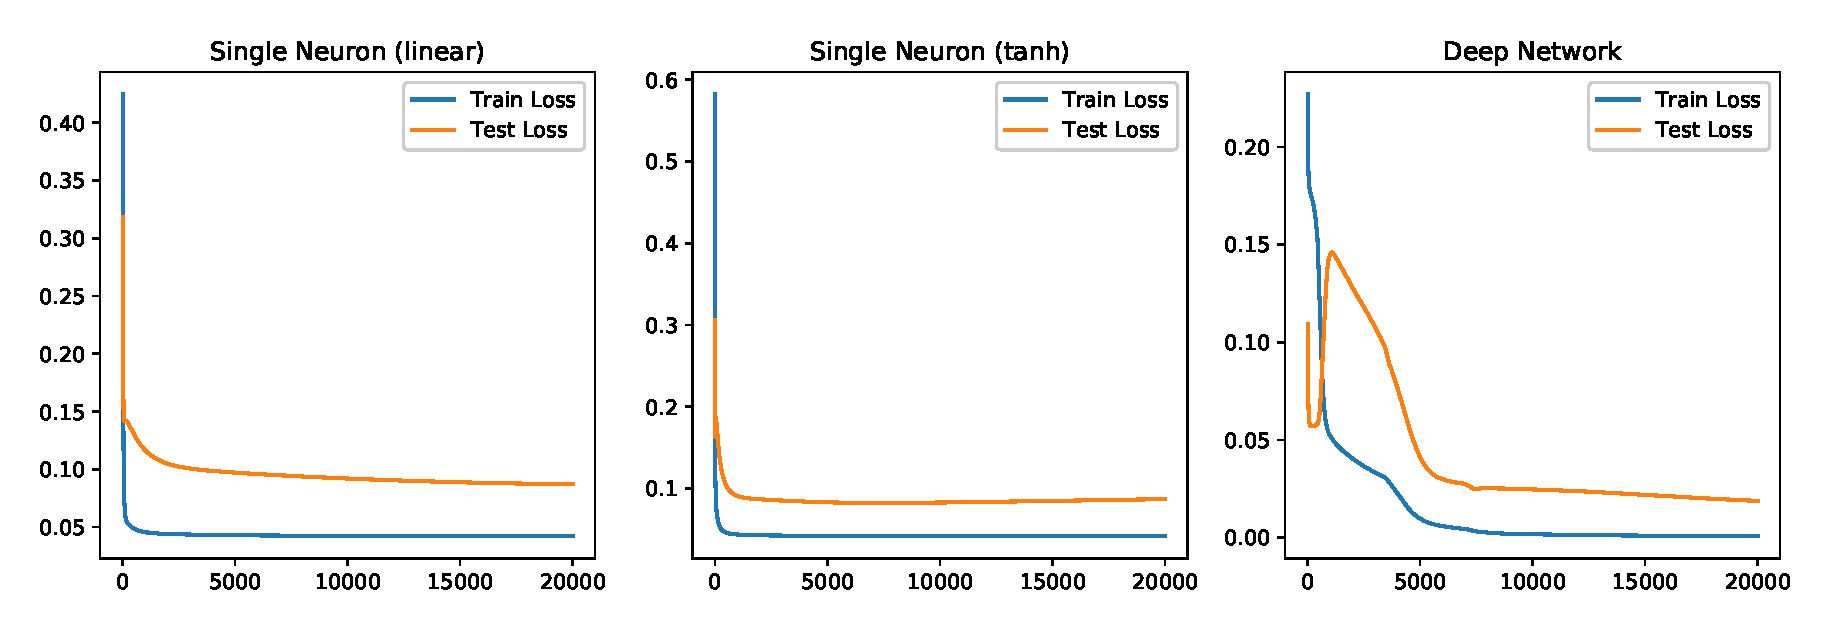
\includegraphics[width=\textwidth]{fig/4/48b2.eps}
     \end{subfigure}
     \caption{Performance of three models, $\sigma^2=0$}
     \label{fig:4_8_b}
\end{figure}\\
When adding a small power of noise $\sigma^2=0.01$, the performance of deep network model is getting worse. Parts of trends are inaccurately captured, resulting in a slightly increased error. Nevertheless, the deep network model still has expressive performance compared with single neuron models.
\begin{figure}[htb]
     \centering
     \begin{subfigure}[b]{0.6\textwidth}
         \centering
         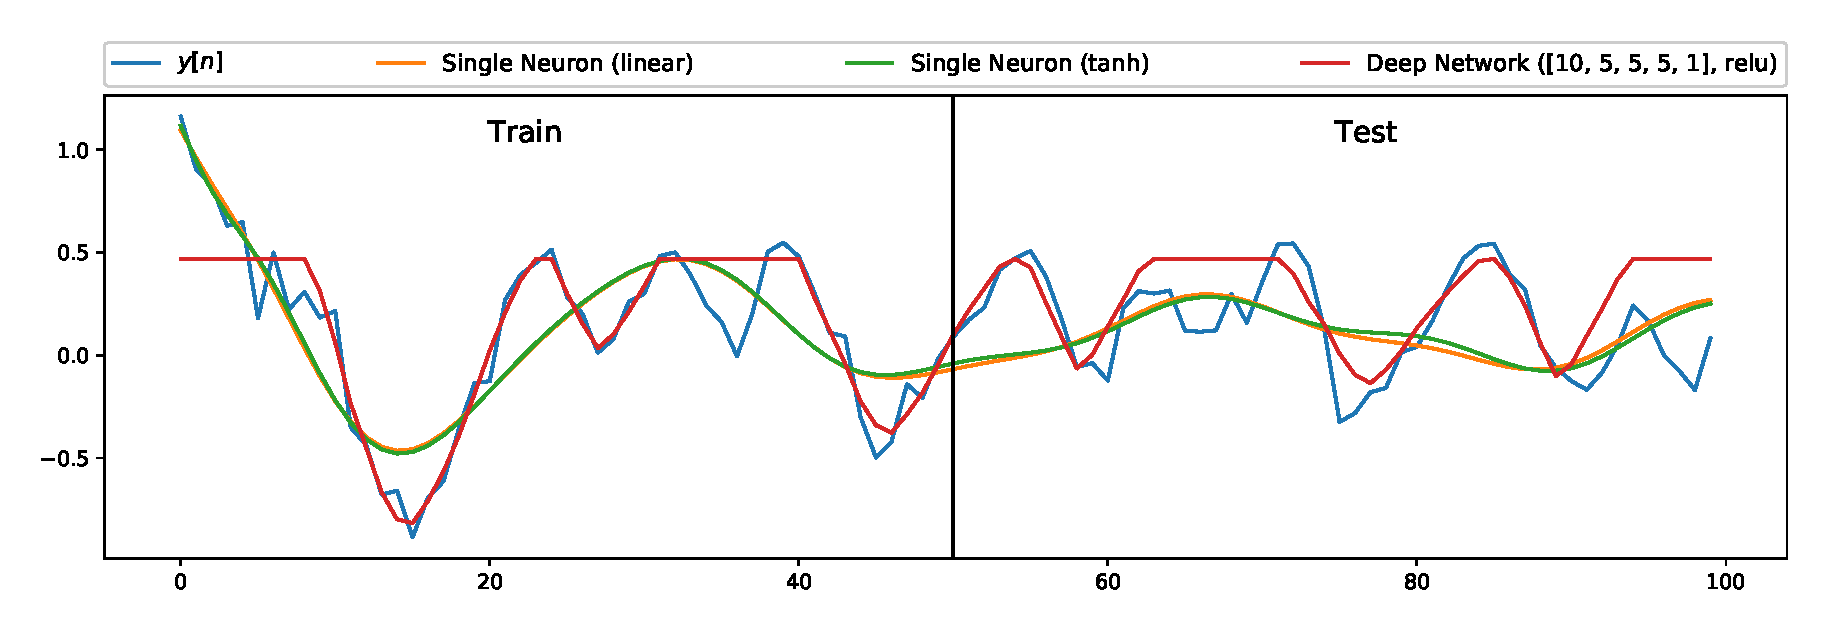
\includegraphics[width=\textwidth]{fig/4/48a1.eps}
     \end{subfigure}
     \begin{subfigure}[b]{0.7\textwidth}
         \centering
         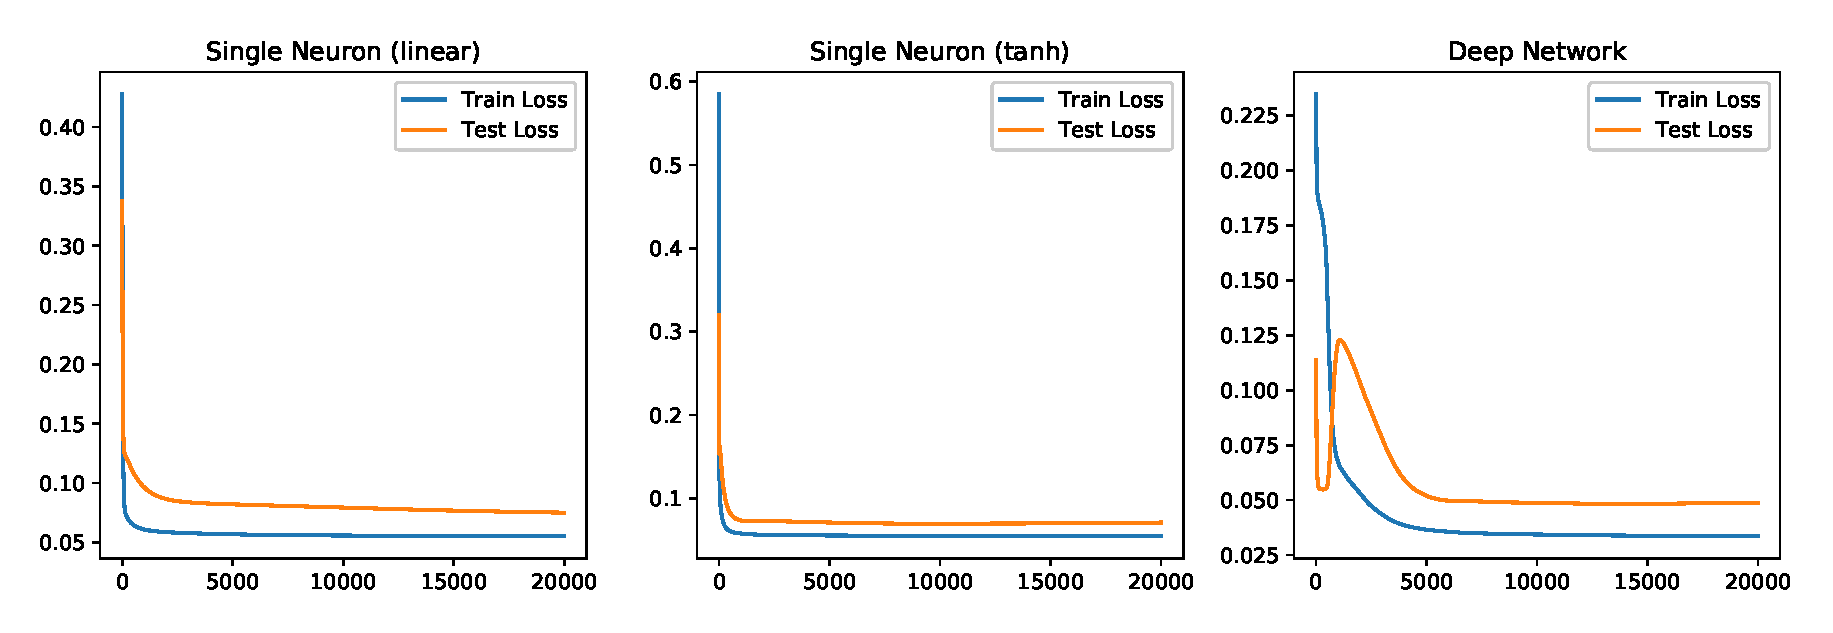
\includegraphics[width=\textwidth]{fig/4/48a2.eps}
     \end{subfigure}
     \caption{Performance of three models, $\sigma^2=0.01$}
     \label{fig:4_8_a}
\end{figure}\\
If the noise power is $\sigma^2=0.2$, the deep network model suffers the problem of over-fitting, which makes the model to predict the noise  sufficiently in training. Thus, the testing error keeps increasing trend.
\begin{figure}[H]
     \centering
     \begin{subfigure}[b]{0.6\textwidth}
         \centering
         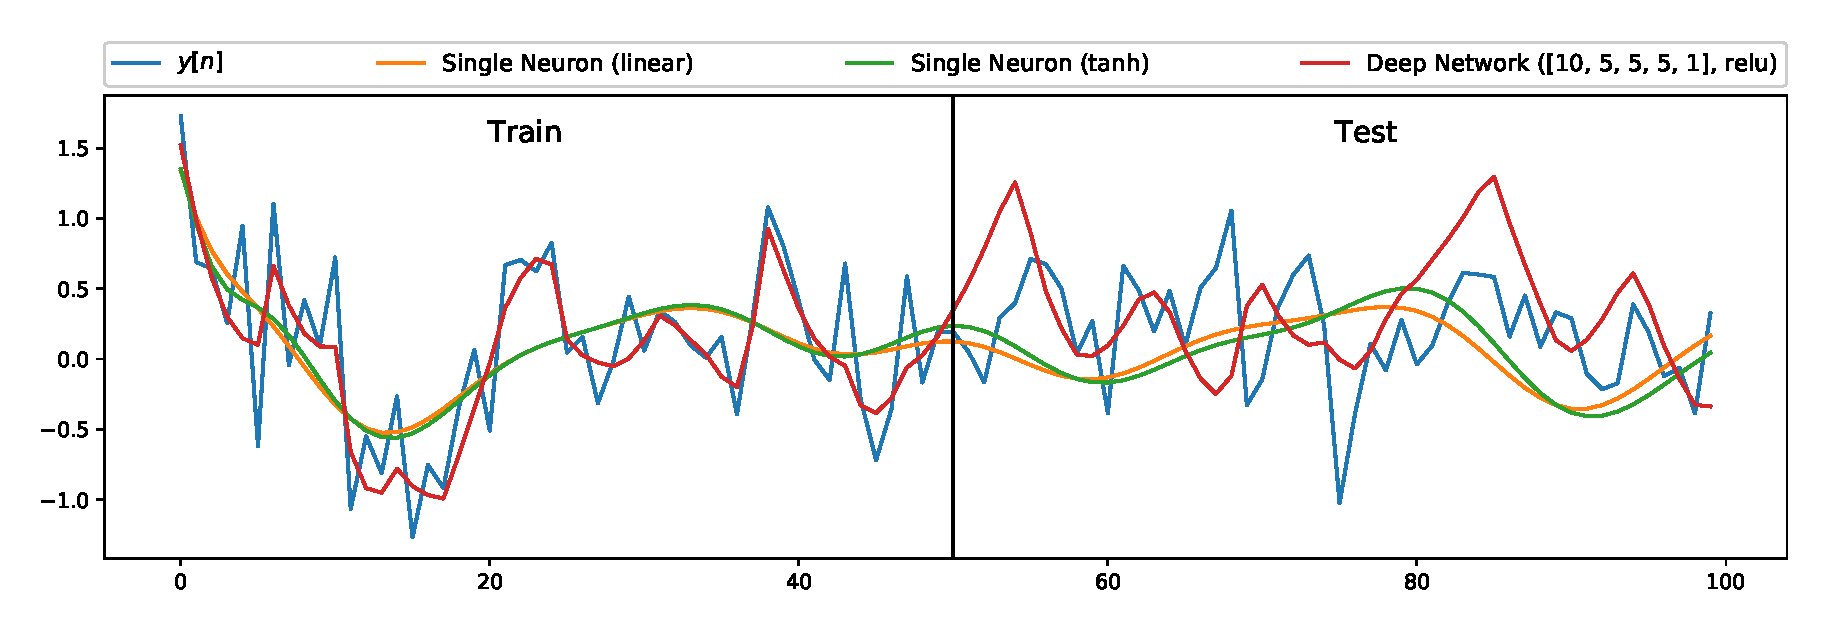
\includegraphics[width=\textwidth]{fig/4/48c1.eps}
     \end{subfigure}
     \begin{subfigure}[b]{0.7\textwidth}
         \centering
         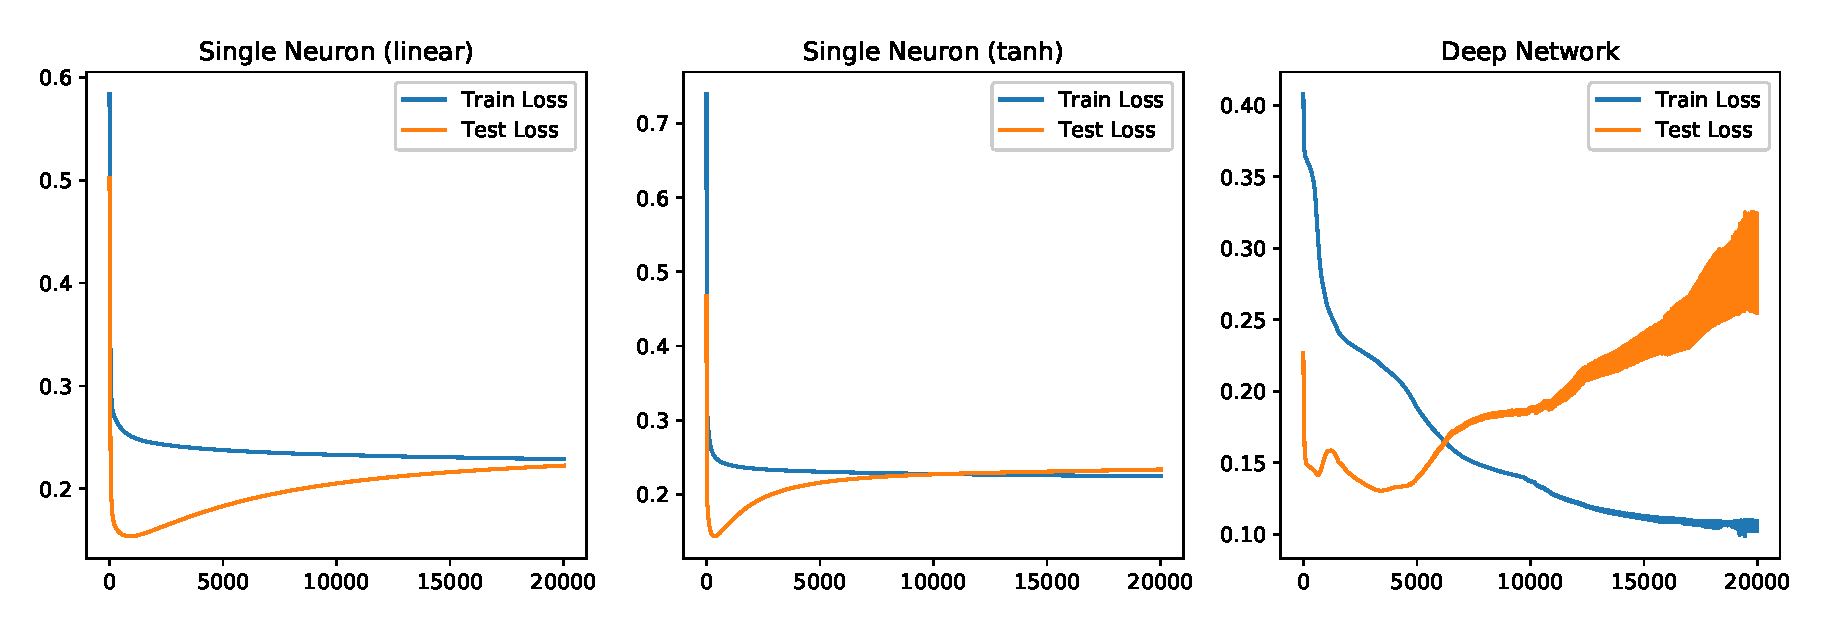
\includegraphics[width=\textwidth]{fig/4/48c2.eps}
     \end{subfigure}
     \caption{Performance of three models, $\sigma^2=0.2$}
     \label{fig:4_8_c}
\end{figure}
\noindent
In summary, by varying the power of noise, the single neuron models perform much robust and stable with less computational cost as well, even if their performances need to be improved. As to the deep network model, it is easily affected by the noise power leading to a unstable performance. Moreover, due to fully-connected with all previous layer inputs and next layer outputs, the computational cost of deep network training is quite large.
